%%%%%%%%%% DOCUMENT STUFF %%%%%%%%%%

\documentclass[10.5pt,letterpaper]{article}
\usepackage{mathtools}
\usepackage{amsmath}
\usepackage{amssymb}
\usepackage{datetime}
\usepackage{setspace}
\usepackage{tikz}
\usepackage[margin=1in]{geometry}
\usepackage{courier}
\usepackage{listings}
\usepackage{mips}
\usepackage{graphicx}
\usepackage{enumitem}
\usepackage{pgfplots}

%%%%%%%%%% FORMATTING %%%%%%%%%%

\newdate{date}{08}{06}{2017}
\spacing{1.5}
\date{\displaydate{date}}
\setcounter{secnumdepth}{0}
\newcommand\tab[1][0.5cm]{\hspace*{#1}}
\newcommand*\circled[1]{\tikz[baseline=(char.base)]{
            \node[shape=circle,draw,inner sep=2pt] (char) {#1};}}
\lstset{language=[mips]Assembler}
\usetikzlibrary{arrows,shapes,automata,petri,positioning,calc}

\tikzset{
    place/.style={
        circle,
        thick,
        draw=black,
        minimum size=6mm,
    },
        state/.style={
        circle,
        thick,
        draw=blue!75,
        fill=blue!20,
        minimum size=6mm,
    },
}

\graphicspath{{images/}}

%%%%%%%%%% CONTENT %%%%%%%%%%

%%%%% COVER PAGE %%%%%

\begin{document}
\title{CS 112: Homework 7}
\author{
	Jonathan Woong\\
	804205763\\
	Spring 2017\\
	Discussion 1A}
\maketitle
\pagebreak

%%%%% PROBLEMS %%%%%

\begin{enumerate}[label=\textbf{Problem \arabic*.}]
\item Consider a simple M/M/1 queueing system that models service of a job in a system. The jobs arrive to be scheduled at rate $\lambda$ jobs per ms. There is a single core capable of serving jobs at the rate of $\mu$ jobs per milli-second. Suppose that the we want the average time spent in the waiting in the queue to be no more than 3 milliseconds. If $\lambda$ = 10 jobs per millisecond, what is the minimum value of $\mu$ for the our requirement to be met?
\[\pi_0 = 1-\rho\]
\[\pi_k = \pi_0(\rho)^k\]
\[\rho=\frac{\lambda}{\mu}\]
\[\text{average number of jobs } = N = \frac{\rho}{1-\rho} = \lambda \cdot T \Rightarrow \text{average time spent } = T = \frac{N}{\lambda}\]
\[T = W + \frac{1}{\mu}\]
\[\text{average waiting time } = W = \frac{\rho}{\lambda(1-\rho)} - \frac{1}{\mu} \leq \frac{1}{20}\]
\[\boxed{\text{Minimum } \mu = 20}\]
\item Customers arrive at a two-server system at a Poisson rate $\lambda$. An arrival finding the system empty is equally likely to enter service with either server. An arrival finding one customer in the system will enter service with the idle server. An arrival finding two others in the system will wait in line for the first free server. An arrival finding three in the system will not enter. All service times are exponential with rate $\mu$, and once a customer is served(by
either server), he departs the system.
	\begin{enumerate}[label=\alph*)]
	\item Define the states.
	\[S = (0,1,2,3) \text{ where state is } S_i \text{ when } i \text{ customers in system}\]
	\item Find the stationary state probability.
	\begin{center}
		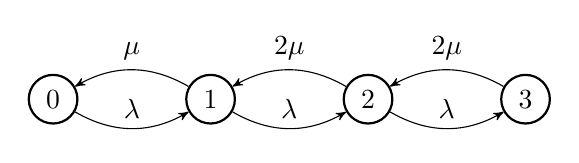
\begin{tikzpicture}[node distance=4cm and 2cm,>=stealth',auto, every place/.style={draw}]
	    \node [place] (0) {0};
	    \node [place] (1) [node distance=2cm,right of=0] {1}; 
	    \node [place] (2) [node distance=2cm,right of=1] {2}; 
	    \node [place] (3) [node distance=2cm,right of=2] {3};   
	    \path [->](0) edge [bend right] node {$\lambda$} (1) 
	    	[<-] edge [bend left] node {$\mu$} (1);
	    \path[->] (1) edge [bend right] node {$\lambda$} (2)
	    	[<-] edge [bend left] node {$2\mu$} (2);
	    \path[->] (2) edge [bend right] node {$\lambda$} (3)
	    	[<-] edge [bend left] node {$2\mu$} (3);         
	\end{tikzpicture}
	\end{center}
	\[\lambda\pi_0 = \mu\pi_1\]
	\[(\lambda+\mu)\pi_1 = \lambda\pi_0 + 2\mu\pi_2\]
	\[(\lambda+2\mu)\pi_2 = \lambda\pi_1 + 2\mu\pi_3\]
	\[2\mu\pi_3 = \lambda\pi_2\]
	\[\pi_0 + \pi_1 + \pi_2 + \pi_3 = 1\]
	\[\pi_0 = \bigg[ 1 + \frac{\lambda}{\mu} + \frac{\lambda^2}{2\mu^2} + \frac{\lambda^3}{4\mu^3} \bigg]^{-1}\]
	\[\boxed{\pi_1 = \frac{\lambda}{\mu}\pi_0, \ \pi_2 = \frac{\lambda^2}{2\mu^2}\pi_0, \ \pi_3 = \frac{\lambda^3}{4\mu^3}\pi_0}\]
	\item Suppose a customer arrives and finds two others in the system. What is the expected times he spends in the system?
	\[T_{\text{system}} = T_{\text{queue}} + T_{\text{service}} = \boxed{\frac{1}{2\mu} + \frac{1}{\mu}}\]
	\item What proportion of customers enter the system?
	\[\boxed{1-\pi_3}\]
	\item What is the average time an entering customer spends in the system?
	\[\text{average \# customers in system} = N = 1 \cdot \pi_1 + 2 \cdot \pi_2 + 3 \cdot \pi_3\]
	\[\lambda_{avg} = (1-\pi_3)\lambda\]
	\[\boxed{T = \frac{N}{\lambda_avg}}\]
	\end{enumerate}
\item A group of $M$ customers frequents a single-server station in the following manner. When a customer arrives, he or she either enters service if the server is free, or joins the queue otherwise. Upon completing service the customer departs the system, but then
returns after an exponential time with rate $\lambda$. All service time are exponentially distributed with rate $\mu$.
	\begin{enumerate}[label=\alph*)]
	\item Define states and set up the balance equations.
	\[S = (0,1,\dots,M) \text{ where state is } S_i \text{ when } i \text{ customers in station}\]
	\begin{center}
		\hspace*{-2cm}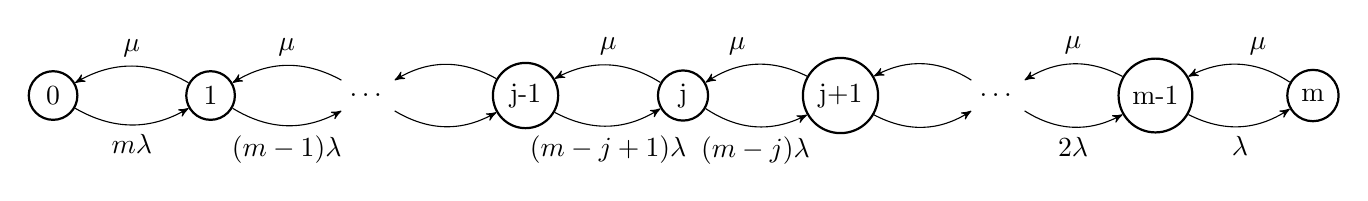
\begin{tikzpicture}[node distance=4cm and 2cm,>=stealth',auto, every place/.style={draw}]
	    \node [place] (0) {0};
	    \node [place] (1) [node distance=2cm,right of=0] {1}; 
	    \node [place,draw=none] (d1) [node distance=2cm, right of=1] {$\dots$};
	    \node [place] (j-1) [node distance=2cm,right of=d1] {j-1}; 
	    \node [place] (j) [node distance=2cm,right of=j-1] {j}; 
	    \node [place] (j+1) [node distance=2cm,right of=j] {j+1}; 
	    \node [place,draw=none] (d2) [node distance=2cm, right of=j+1] {$\dots$};  
	    \node [place] (m-1) [node distance=2cm,right of=d2] {m-1};
	    \node [place] (m) [node distance=2cm,right of=m-1] {m};
	    \path [->](0) edge [bend right] node [below] {$m\lambda$} (1) 
	    	[<-] edge [bend left] node {$\mu$} (1);
	    \path[->] (1) edge [bend right] node [below] {$(m-1)\lambda$} (d1)
	    	[<-] edge [bend left] node {$\mu$} (d1);
	    \path[->] (d1) edge [bend right] node [below] {} (j-1)
	    	[<-] edge [bend left] node {} (j-1);  
	    \path[->] (j-1) edge [bend right] node [below] {$(m-j+1)\lambda$} (j)
	    	[<-] edge [bend left] node {$\mu$} (j);  
	    \path[->] (j) edge [bend right] node [below] {$(m-j)\lambda$} (j+1)
	    	[<-] edge [bend left] node {$\mu$} (j+1); 
	    \path[->] (j+1) edge [bend right] node [below] {} (d2)
	    	[<-] edge [bend left] node {} (d2);
	    \path[->] (d2) edge [bend right] node [below] {$2\lambda$} (m-1)
	    	[<-] edge [bend left] node {$\mu$} (m-1);  
	    \path[->] (m-1) edge [bend right] node [below] {$\lambda$} (m)
	    	[<-] edge [bend left] node {$\mu$} (m);      
	\end{tikzpicture}
	\end{center}
	\fbox{\parbox{\widthof{$[(m-J)\lambda+\mu]\pi_J = (m-K+1)\lambda\pi_{J-1}+\mu\pi_{J+1}, \ 1 \leq J \leq m-1$}}{
	\[m\lambda\pi_0 = \mu\pi_1\]
	\[[(m-J)\lambda+\mu]\pi_J = (m-K+1)\lambda\pi_{J-1}+\mu\pi_{J+1}, \ 1 \leq J \leq m-1\]
	\[\mu\pi_m = \lambda\pi_{m-1}\]
	\[\sum_{J=0}^{m}\pi_J = 1\]
	}}
	\item The average rate at which customers enter the station. (Suppose steady state probability $\pi$ = ($\pi_0$, $\pi_1$, $\dots$ , $\pi_M$))
	\[\boxed{\lambda_a = \sum_{J=0}^{m}\pi_J\lambda_J = \sum_{J=0}^{m}\pi_J(m-J)\lambda}\]
	\item The average time that a customer spends in the station per visit. (Suppose steady state probability $\pi$ = ($\pi_0$, $\pi_1$, $\dots$ , $\pi_M$)
	\[\boxed{W = \frac{N}{\lambda_a} = \frac{\sum_{J=0}^m\pi_J(m-J)\lambda}{\sum_{J=0}^m(m-J)\lambda\pi_J}}\]
	\end{enumerate}
\item Consider a bank with a single teller. An average of 45 customers per hour arrive at the bank and wait in a single line for until the teller idle. The average time it takes to serve a customer is 1.2 minutes. Assume that inter-arrival times and service times are exponentially distributed. Determine:
	\begin{itemize}
	\item The expected number of customers present in the bank.
	\[\lambda = 45, \ \mu = \frac{60}{1.2}=50\]
	\[\rho = \frac{\lambda}{\mu} = \frac{45}{50} = 0.9\]
	\[\boxed{N = \frac{\rho}{1-\rho} = \frac{0.9}{1-0.9} = 9}\]
	\item The expected length of a time a a customer spends in the bank.
	\[N = \lambda T \Rightarrow \boxed{T = \frac{N}{\lambda} = \frac{9}{45} = 0.2 \text{ hours} = 12 \text{ minutes}}\]
	\item The expected length of a time a a customer waits in the line.
	\[T = \frac{1}{\mu} + W \Rightarrow \boxed{W = T - \frac{1}{\mu} = 0.2 - \frac{1}{50} = 0.18 \text{ hours} = 10.6 \text{ minutes}}\]
	\item The proportion of time the teller will be busy.
	\[\boxed{\rho = \frac{\lambda}{\mu} = \frac{45}{50} = 0.9}\]
	\end{itemize}
\item Data request arrive at a cache of a multi-core processor of 60 cores in a Poisson distributed arrival rate of 25 cache line requests per cycle. Cache reply rate is exponentially distributed with an average data supply rate of 2 clock cycle per request for all 60 cores.
Calculate the mean number of data request waiting in the buffer, the mean waiting time, the mean number of data requests in the system, the mean time a data request in the system and the utilization factor.\\
\fbox{\parbox{\textwidth}{\[\lambda = 25, \ \mu = \frac{1}{2} = 0.5, \ m=60\]
\[\rho = \frac{\lambda}{m\mu} = \frac{25}{60(0.5)} = \frac{25}{30}\]
\[p_0 = \bigg[\frac{(m\rho)^m}{m!(1-\rho)}+\sum_{i=0}^{m-1}\frac{(m\rho)^i}{i!}\bigg]^{-1} = \bigg[\frac{(60\times\frac{25}{30})^{60}}{60!(1-\frac{25}{30})}+\sum_{i=0}^{59}\frac{(60\times\frac{25}{30})^i}{i!}\bigg]^{-1} = 1.8755 \times 10^{-22}\]
\[P(\geq m \text{ requests}) = \zeta = \frac{(m\rho)^m}{m!(1-\rho)}p_0 = \frac{(60\times\frac{25}{30})^{60}}{60!(1-\frac{25}{30})}(1.8755 \times 10^{-22}) = 0.1173\]
\[\text{mean \# requests waiting in buffer} = N_q = m\rho = (60\times\frac{25}{30}) = 50 \text{ requests}\]
\[\text{mean waiting time} = W_q = \frac{N_q}{\lambda} = \frac{50}{25} = 2 \text{ cycles}\]
\[\text{mean \# requests in system} = N = N_q + N_s = m\rho + \frac{\rho\zeta}{1-\rho} = (60\times\frac{25}{30})+\frac{\frac{25}{30}\times0.1173}{1-\frac{25}{30}} = 50.5865\]
\[\text{mean time in system} = T = W_q + \frac{1}{\mu} = 2 + \frac{1}{0.5} = 4 \text{ cycles}\]
\[\text{utilization factor} = U = \frac{\lambda}{m\mu} = \frac{25}{30}\]}}
\item Consider a simple M/M/1 queuing system, modeling the execution of jobs by a CPU. The jobs arrive at a rate of $\lambda$ jobs per millisecond and the single CPU is capable of executing jobs at the rate of $\mu$ jobs per millisecond.
	\begin{enumerate}[label=\alph*)]
	\item Suppose we want the average time $T$ spent in system by a job (waiting time + execution time) to be no more than 10 milliseconds. If the CPU can handle jobs at the rate of $\mu$ = 3 jobs per millisecond, what is the maximum job-arrival rate $\lambda$ that the system can handle while meeting the constraint on $T$?
	\[\rho = \frac{\lambda}{\mu}\]
	\[N = \frac{\rho}{1-\rho} = \lambda \cdot T \Rightarrow T = \frac{N}{\lambda}\]
	\[T = \frac{\rho}{\lambda(1-\rho)} = \frac{\lambda}{\mu\lambda(1-\frac{\lambda}{\mu})} = \frac{1}{\mu(1-\frac{\lambda}{\mu})}\] 
	\[\lambda = \mu - \frac{1}{T} = 3 - \frac{1}{10} = \boxed{2.9}\]
	\item Calculate the utilization factor $\rho$ and the average number of jobs $N$ in the system, assuming that $\lambda$ is equal to the value found in part a).\\
	\fbox{\parbox{\textwidth}{\[\rho = \frac{\lambda}{\mu} = \frac{2.9}{3}\]
	\[N = \frac{\rho}{1-\rho} = \frac{\frac{2.9}{3}}{1-\frac{2.9}{3}} = 29 \text{ jobs}\]}}
	\item  Suppose we want CPU to be busy 99.5\% of the time. At what rate $\lambda$ should jobs be fed into the system in order to satisfy this requirement? What are the values of $T$ and $N$ in this case? What is the average amount of time spent waiting in queue in this case?\\
	\fbox{\parbox{\textwidth}{\[\rho = \frac{\lambda}{\mu} \Rightarrow \lambda = \rho\mu = 0.995 \times 3 = 2.985\]
	\[T = \frac{\rho}{\lambda(1-\rho)} = \frac{0.995}{2.985(1-0.995)} = \frac{200}{3}\]
	\[N = T\cdot\lambda = \frac{200}{3} \times 2.985 = 199\]
	\[W = T - \frac{1}{\mu} = \frac{200}{3} - \frac{1}{3} = \frac{199}{3} \text{ milliseconds} \]}}
	\end{enumerate}
\item A computing server has a finite buffer with size = 6 requests (excluding the one being handled). Assuming that the arrival rate of incoming requests is Poisson with average 9 requests per minute, and handling one request takes exponentially distributed service time with average 8 seconds. Answer the following questions:
	\begin{itemize}
		\item What is the average number of request in the the server?, and what is the average number of requests waiting?
		\[K = 6,\ m = 1,\ \lambda = 9,\ \mu = \frac{60}{8} = 7.5\]
		\[\frac{\lambda}{\mu} = \frac{9}{7.5} = 1.2\]
		\[p_0 = \frac{1-\frac{\lambda}{\mu}}{1-\bigg(\frac{\lambda}{\mu}\bigg)^{K+1}} = \frac{1-1.2}{1-1.2^7} = 0.0774\]
		\[p_k = p_0\bigg(\frac{\lambda}{\mu}\bigg)^k=0.0774\bigg(\frac{9}{7.5}\bigg)^k = 0.0774(1.2)^k\]\\
		\fbox{\parbox{\textwidth}{\[N = \sum_{i=1}^{K}ip_i = 3.7098 \text{ requests}\]
		\[N_q = \sum_{i=m+1}^{K}(i-m)p_i = \sum_{i=2}^{K}(i-1)p_i = 2.7873 \text{ requests}\]}}
		\item If the fee of one request is \$0.25 and the server works 12 hours a day, how much money is gained on average each day? and how much gain is lost (due to discarded requests)?
		\[\text{effective arrival rate}=\widetilde{\lambda} = \sum_{i=0}^{K-1}\lambda p_i = \lambda(1-p_K) = 9(1-0.2312) = 6.9193\]
		\[\widetilde{\lambda} = 6.9193 \text{ requests/minute} = 415.1592 \text{ requests/hour} \Rightarrow 4981.9108 \text{ requests/day}\]
		\[\boxed{\text{daily gain} = 4981.9108 \text{ requests/day} \times \$0.25 \text{/request} = \$1245.48 \text{ per day}}\]
		\[\text{loss rate} = \lambda - \widetilde{\lambda} = 9 - 6.9193 = 2.0807 \text{ per minute}\]
		\fbox{\parbox{\textwidth}{\begin{equation*}\begin{split}
		\text{daily loss} & = 2.0807 \text{ per minute} \times \$0.25 \text{/request}\\
		& = 124.842 \text{ per hour}  \times \$0.25 \text{/request}\\
		& = 1498.104 \text{ per day} \times \$0.25 \text{/request}= \$374.53 \text{ per day}\end{split}\end{equation*}}}
		\item On average, how long does a request have to wait until being handled?
		\[T = \frac{N}{\widetilde{\lambda}} = \frac{2.7873}{6.9193} = 0.4028 \text{ minutes}\]
		\[\boxed{W = T - \frac{1}{\mu} = 0.4028 - \frac{1}{7.5} = 0.2645 \text{ minutes}}\]
		\item The server administrators decided that they should buy another server, if the old server works more than 85\% of time. should they buy a new one?
		\[U = \frac{\widetilde{\lambda}}{\mu} = \frac{6.9193}{7.5} = 0.9223\]
		\fbox{\parbox{\textwidth}{The current server works 92.23\% of the time, so the server should be replaced if there is the possiblity of it working only 85\% of the time.}}
	\end{itemize}
\item Consider a computing cluster with two servers. An average of 90 requests per hour are received and they are placed in a single buffer until one of the servers becomes free to handle it (FCFS). The average time it takes to serve a customer is 1.2 minutes. Assuming that inter-arrival times and service times are exponential. Determine:
	\begin{itemize}
	\item The probability that there are no requests in the system.
	\[m=2,\ \lambda = 90,\ \mu=\frac{60}{1.2}=50\]
	\[\rho = \frac{\lambda}{m\mu} = \frac{90}{2\times50} = 0.9\]
	\[\boxed{p_0 = \bigg[\frac{(m\rho)^m}{m!(1-\rho)}+\sum_{i=0}^{m-1}\frac{(m\rho)^i}{i!}\bigg]^{-1} = \bigg[1+\frac{(2\times0.9)^2}{2!(1-0.9)}+(2\times0.9)\bigg]^{-1} = 0.0526}\]
	\item The expected number of requests in the system.
	\[P(\geq m \text{ requests}) = \zeta = \frac{(m\rho)^m}{m!(1-\rho)}p_0 = \frac{(2\times0.9)^2}{2!(1-0.9)}0.0526 = 0.8521\]
	\[\boxed{N = N_q + N_s = m\rho + \frac{\rho\zeta}{1-\rho} = (2\times0.9)+\frac{0.9\times0.8521}{1-0.9} = 9.2489}\]
	\item The expected time a request stays waiting in the buffer.
	\[\boxed{W = \frac{\rho}{m\mu(1-\rho)} = \frac{0.9}{2\times50\times(1-0.9)} = 0.09 \text{ hours} = 5.4 \text{ minutes}}\]
	\end{itemize}
\item UCLA computer science department receives an average of 10 application requests for masters degree in computer science. All requests are reviewed for acceptance and each request has a probability of 0.7 of getting accepted to the program. The MSc program takes 2 years on average. Assuming that Poisson arrival for the incoming requests and exponential time for the degree length.
	\begin{itemize}
	\item What is the probability that no students in the program?
	\[\lambda = 10\times0.7 = 7, \ T = 2\]
	\[T = \frac{1}{\mu-\lambda} \Rightarrow \mu = \frac{1}{T} + \lambda = \frac{1}{2} + 7 = 7.5\]
	\[\rho = \frac{\lambda}{\mu} = \frac{7}{7.5} = 0.9333\]
	\[\boxed{p_0 = 1-\rho = 1-0.9333 = 0.0667}\]
	\item What is average number of students in the program each year?
	\[\boxed{N = \lambda \cdot T = 7 \times 2 = 14 \text{ students}}\]
	\end{itemize}
\end{enumerate}
\end{document}